%!TeX root = ../main.tex

\section{Data}
\subsection{Dataset}
The data of the experiment are divided into two groups of images, one used for the training of the autoencoder and another one for the testing. The images represent four buildings from different points of view. In the training group there are images of Portello and Castle (some of them are reported in fig. \ref{fig:portello} and fig. \ref{fig:castle}), while in the group of the testing images there are images of fountain and Tiso, some of them reported in fig. \ref{fig:fountain} and fig. \ref{fig:tiso}.

\begin{figure}[H]
     \centering
     \begin{subfigure}[b]{0.3\textwidth}
         \centering
         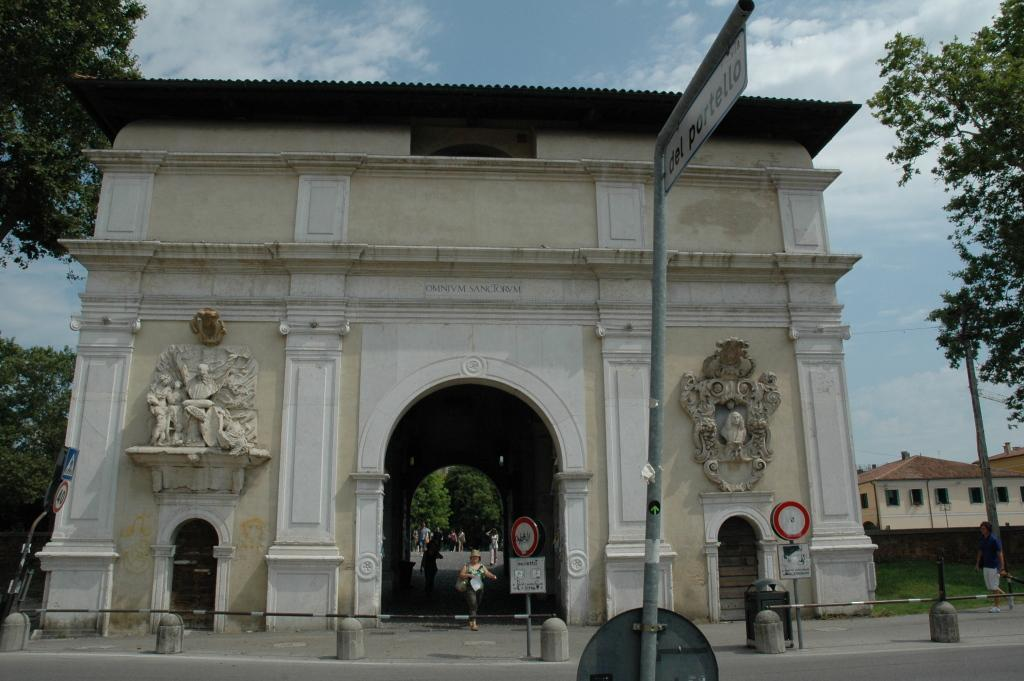
\includegraphics[width=\textwidth]{../../Project_3DAR/images/Training/portelloDataset/img000.jpg}
     \end{subfigure}
     \hfill
     \begin{subfigure}[b]{0.3\textwidth}
         \centering
         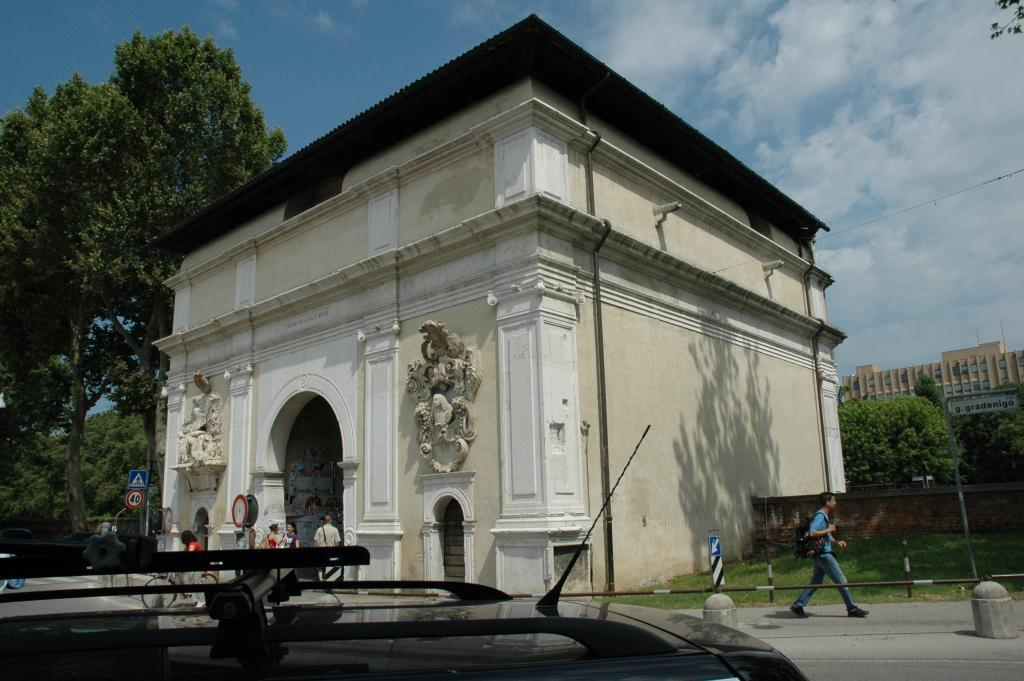
\includegraphics[width=\textwidth]{../../Project_3DAR/images/Training/portelloDataset/img013.jpg}
     \end{subfigure}
     \hfill
     \begin{subfigure}[b]{0.3\textwidth}
         \centering
         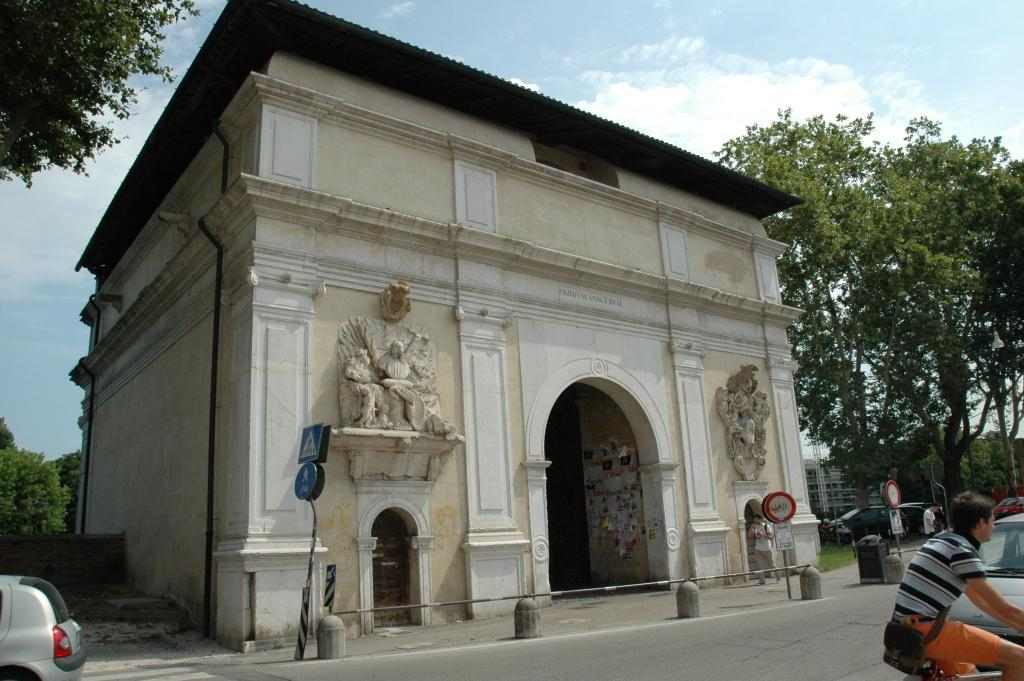
\includegraphics[width=\textwidth]{../../Project_3DAR/images/Training/portelloDataset/img030.jpg}
     \end{subfigure}
        \caption{samples from Portello dataset.}
        \label{fig:portello}
\end{figure}

\begin{figure}[H]
     \centering
     \begin{subfigure}[b]{0.3\textwidth}
         \centering
         \includegraphics[width=\textwidth]{../../Project_3DAR/images/Training/castle/0004.jpg}
     \end{subfigure}
     \hfill
     \begin{subfigure}[b]{0.3\textwidth}
         \centering
         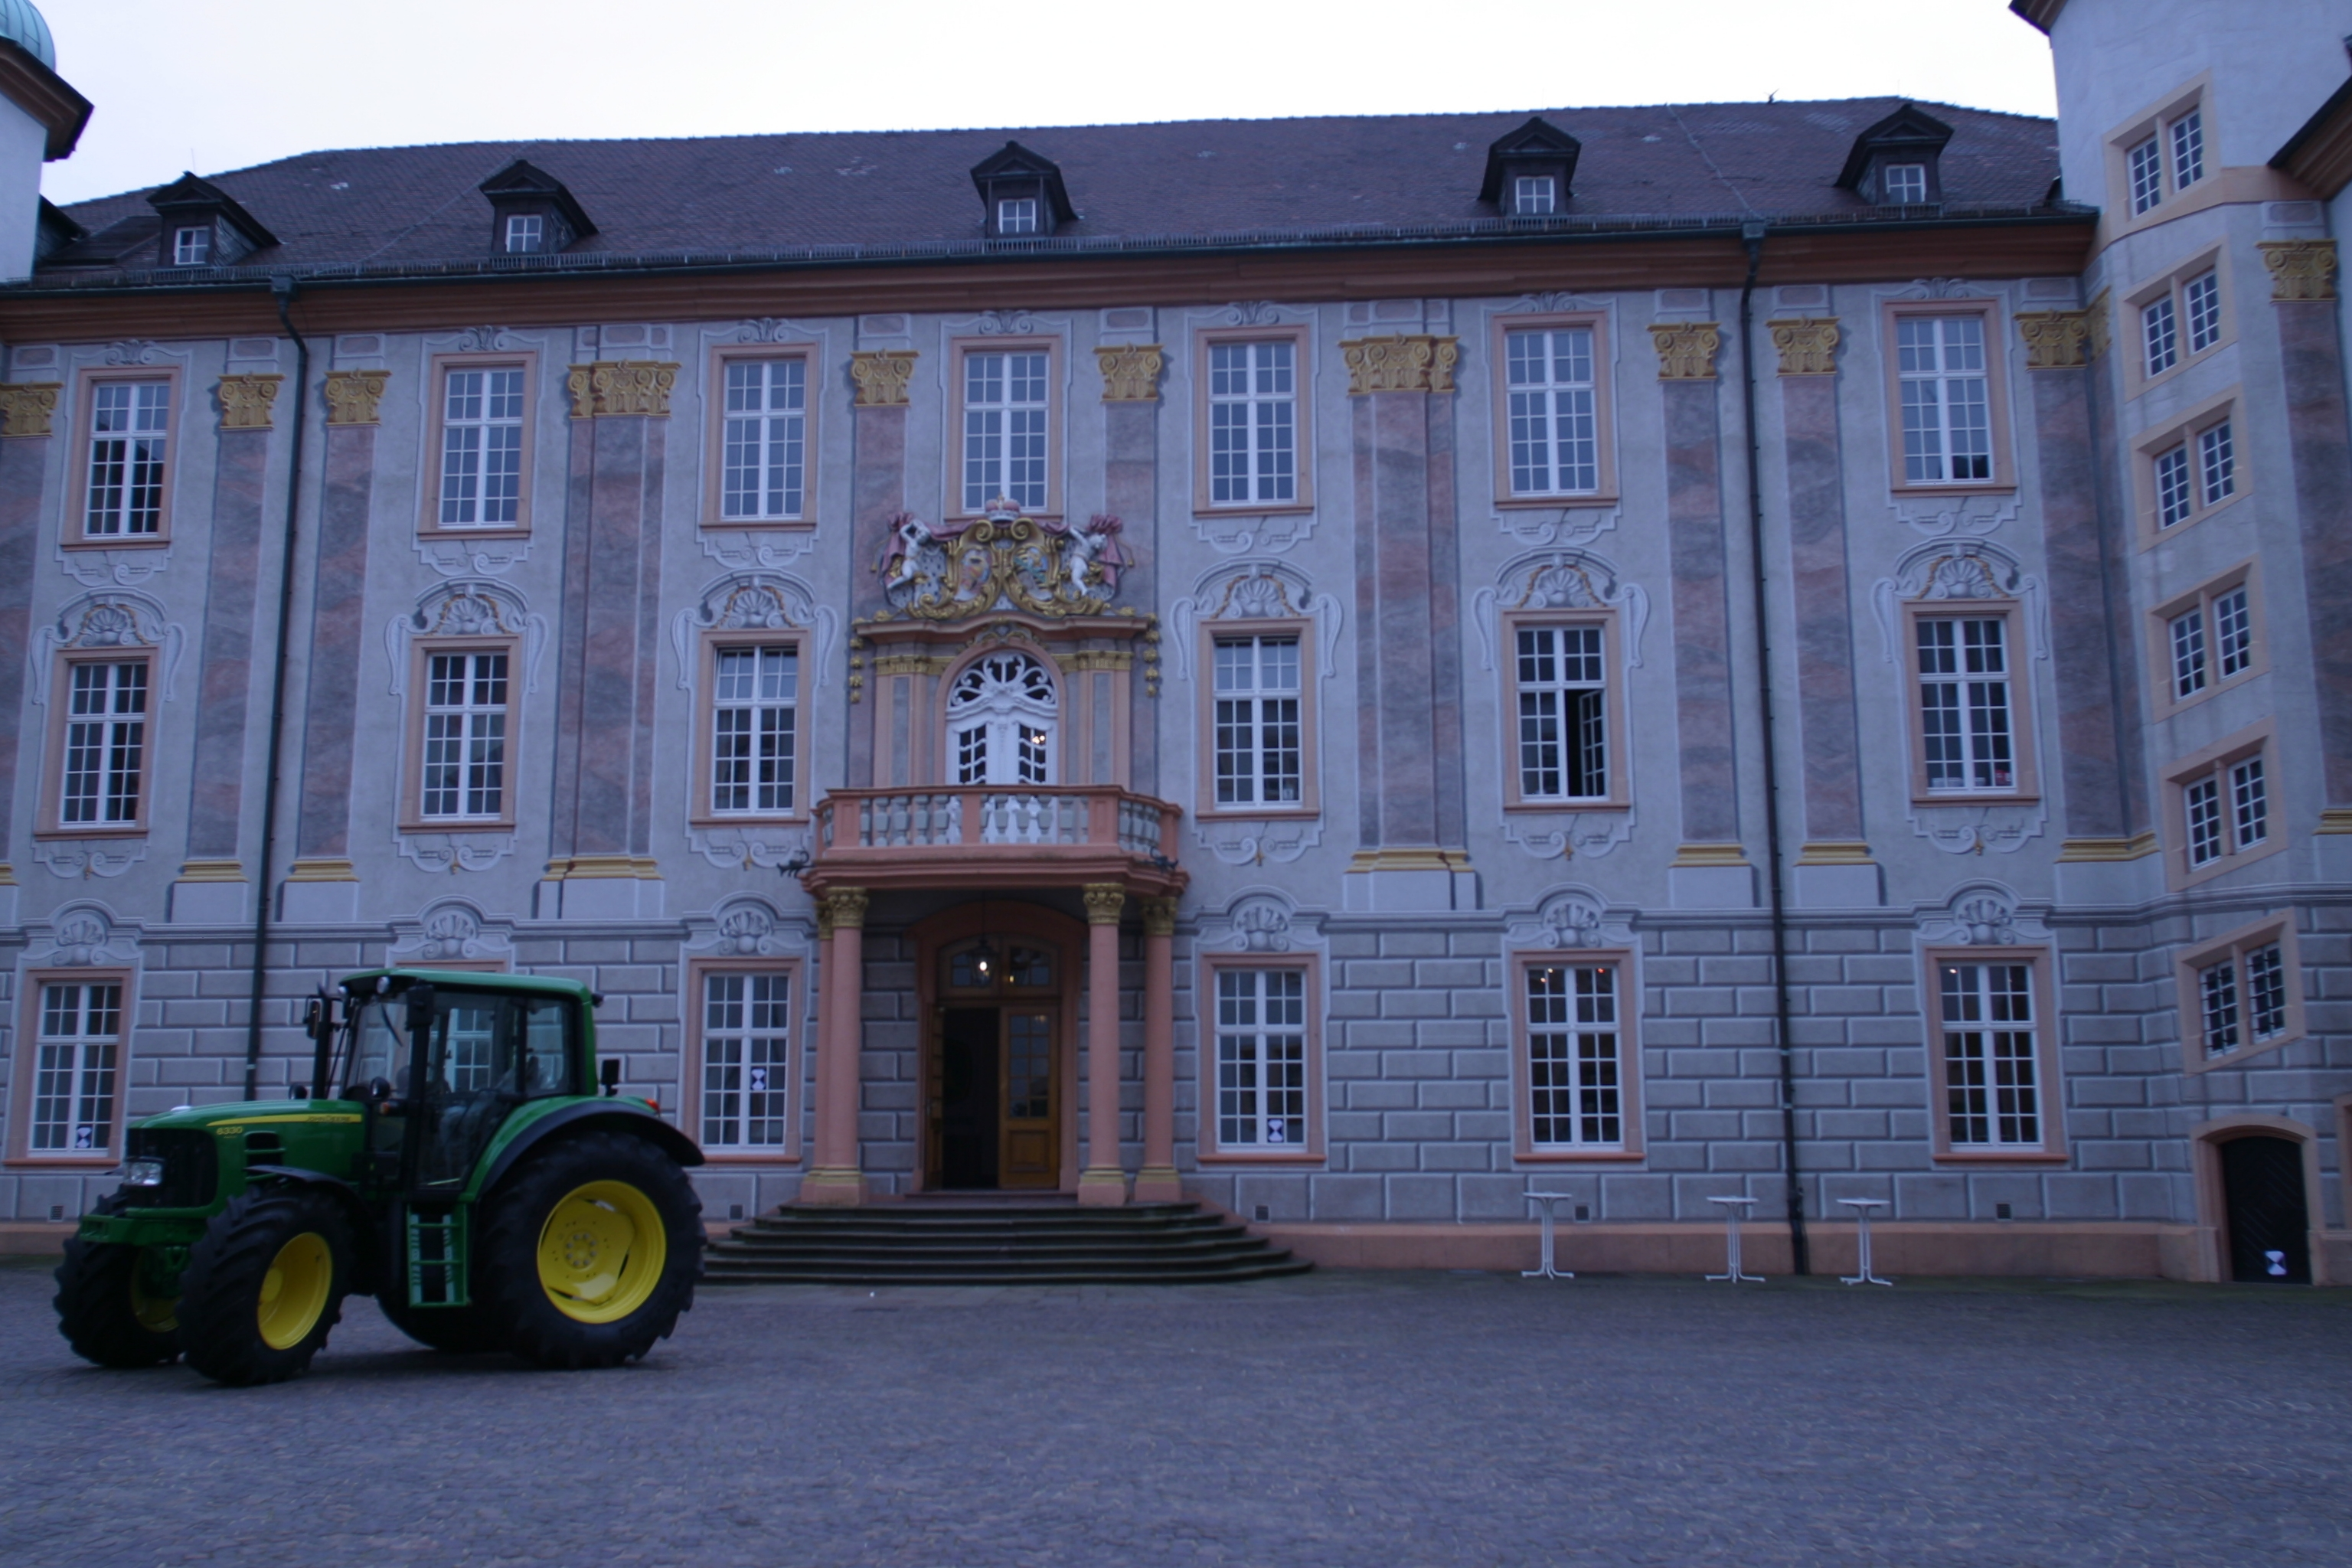
\includegraphics[width=\textwidth]{../../Project_3DAR/images/Training/castle/0010.jpg}
     \end{subfigure}
     \hfill
     \begin{subfigure}[b]{0.3\textwidth}
         \centering
         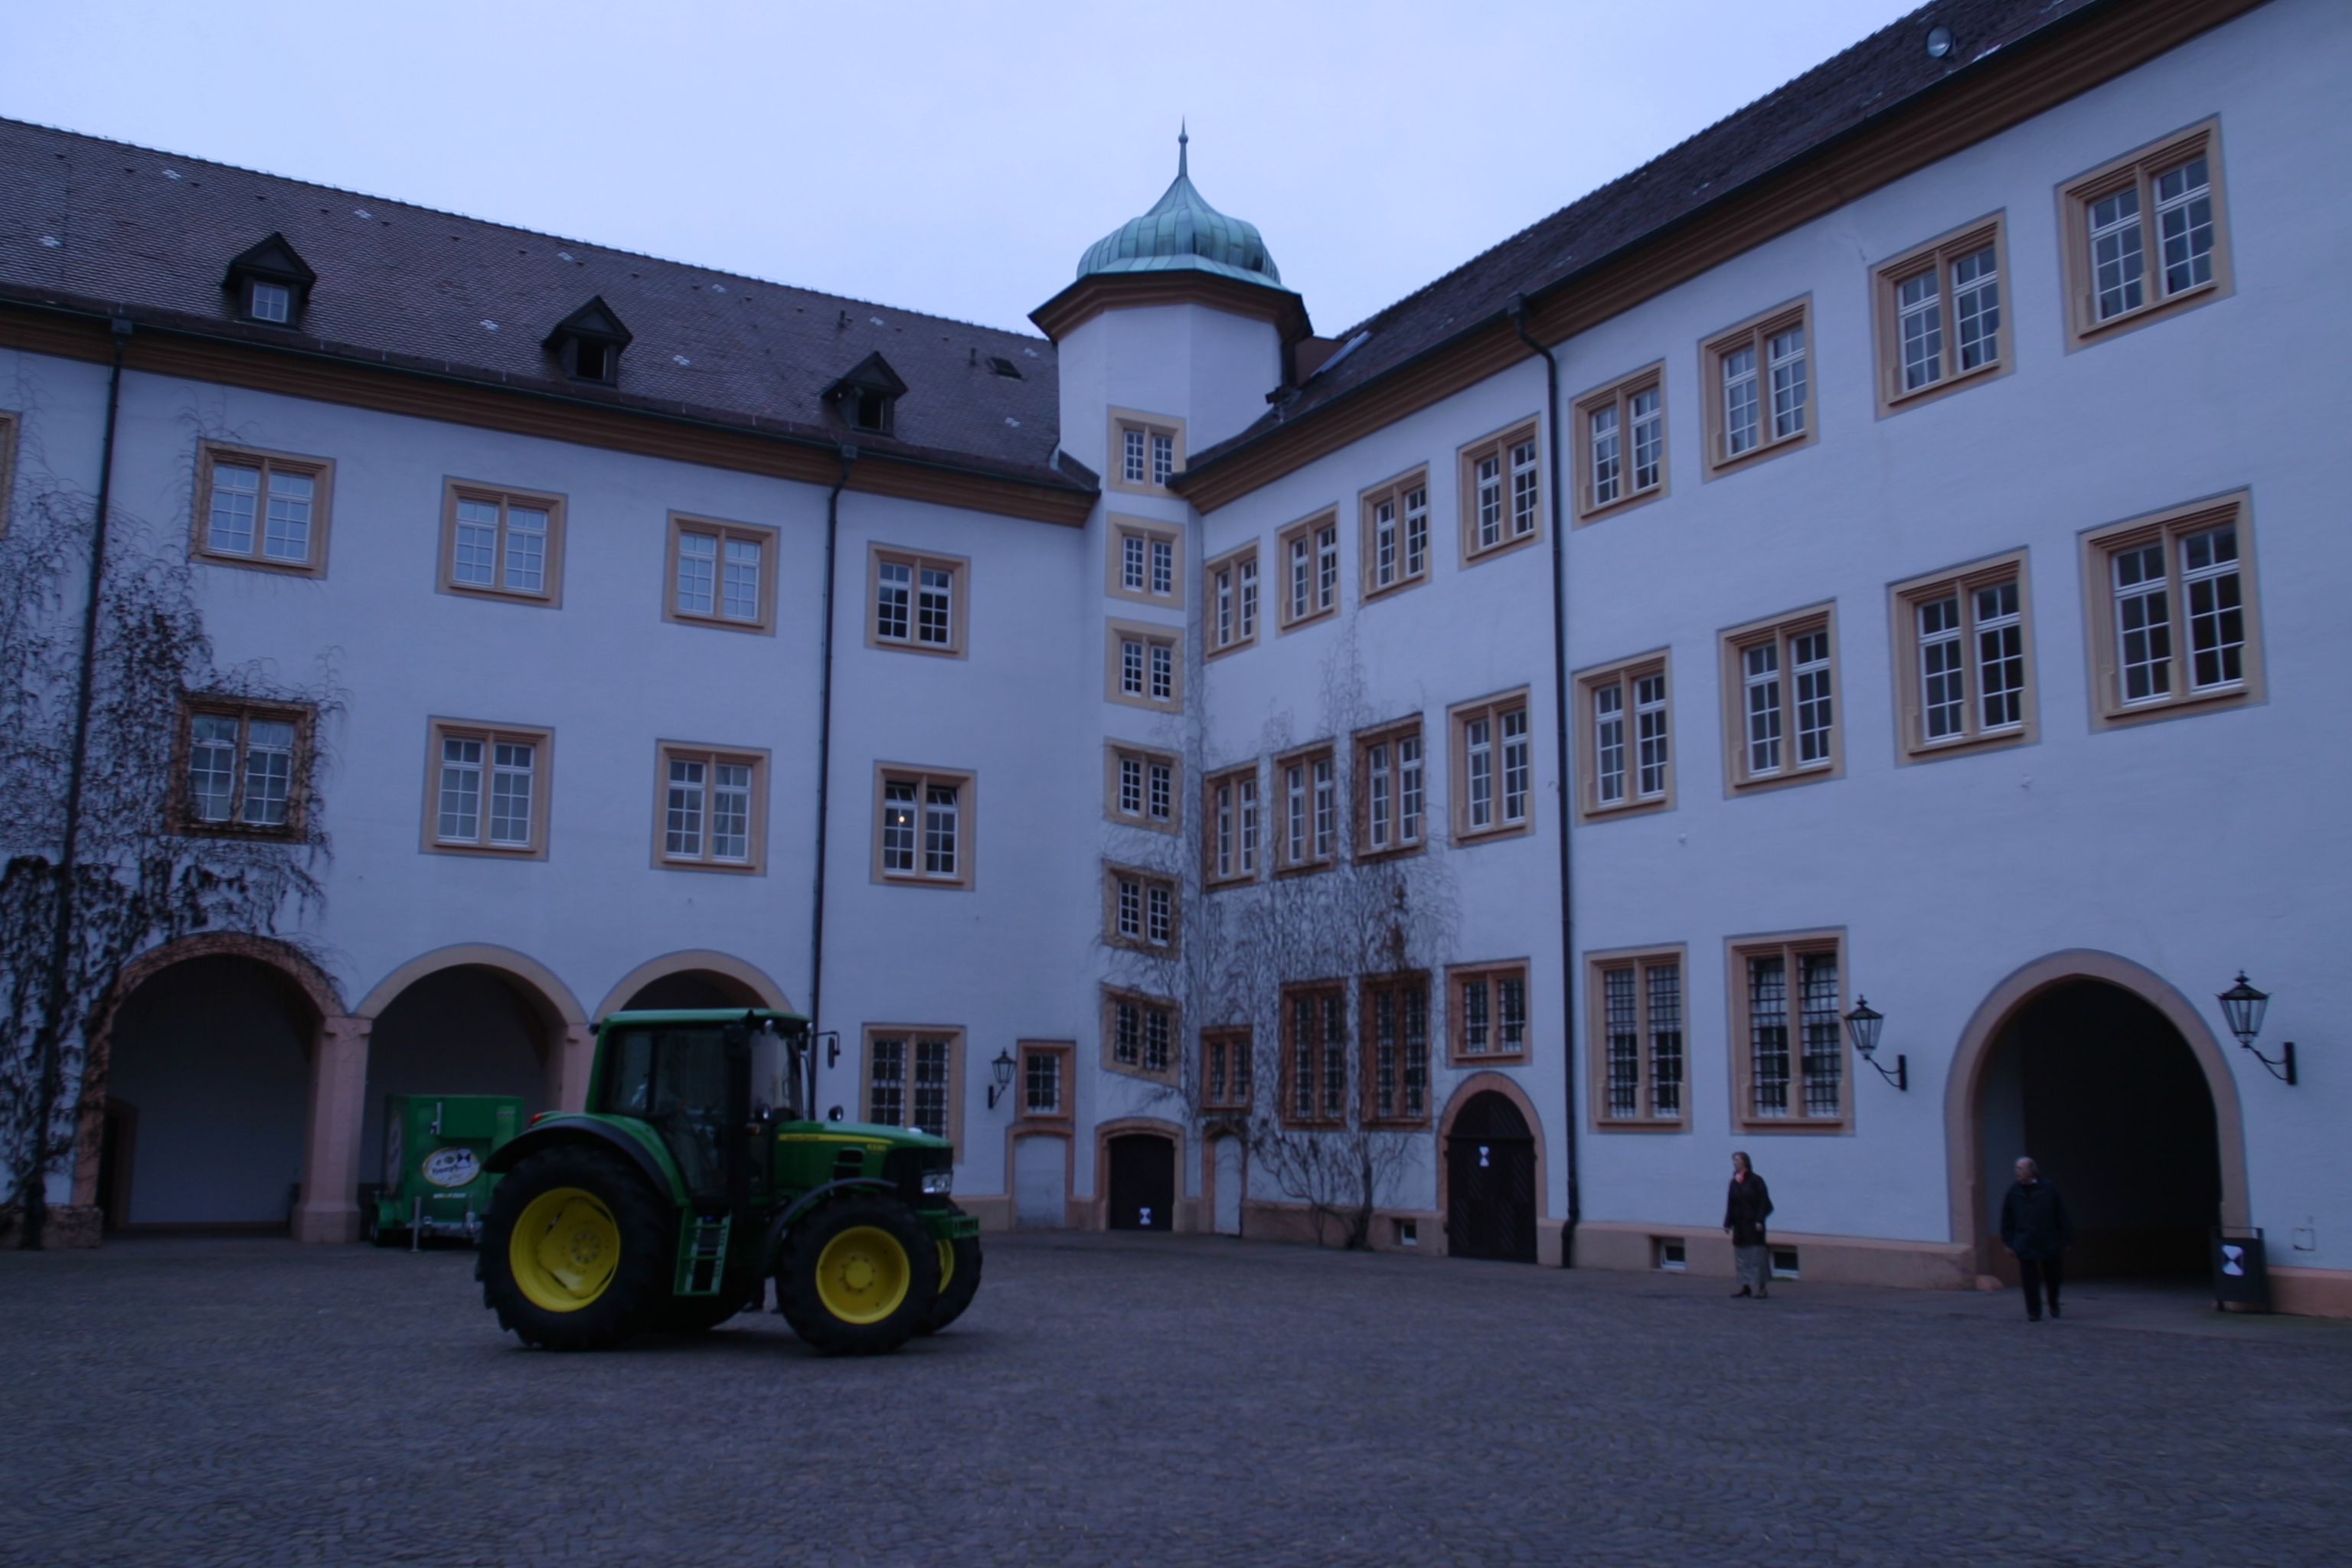
\includegraphics[width=\textwidth]{../../Project_3DAR/images/Training/castle/0028.jpg}
     \end{subfigure}
        \caption{samples from castle dataset.}
        \label{fig:castle}
\end{figure}

\begin{figure}[H]
     \centering
     \begin{subfigure}[b]{0.3\textwidth}
         \centering
         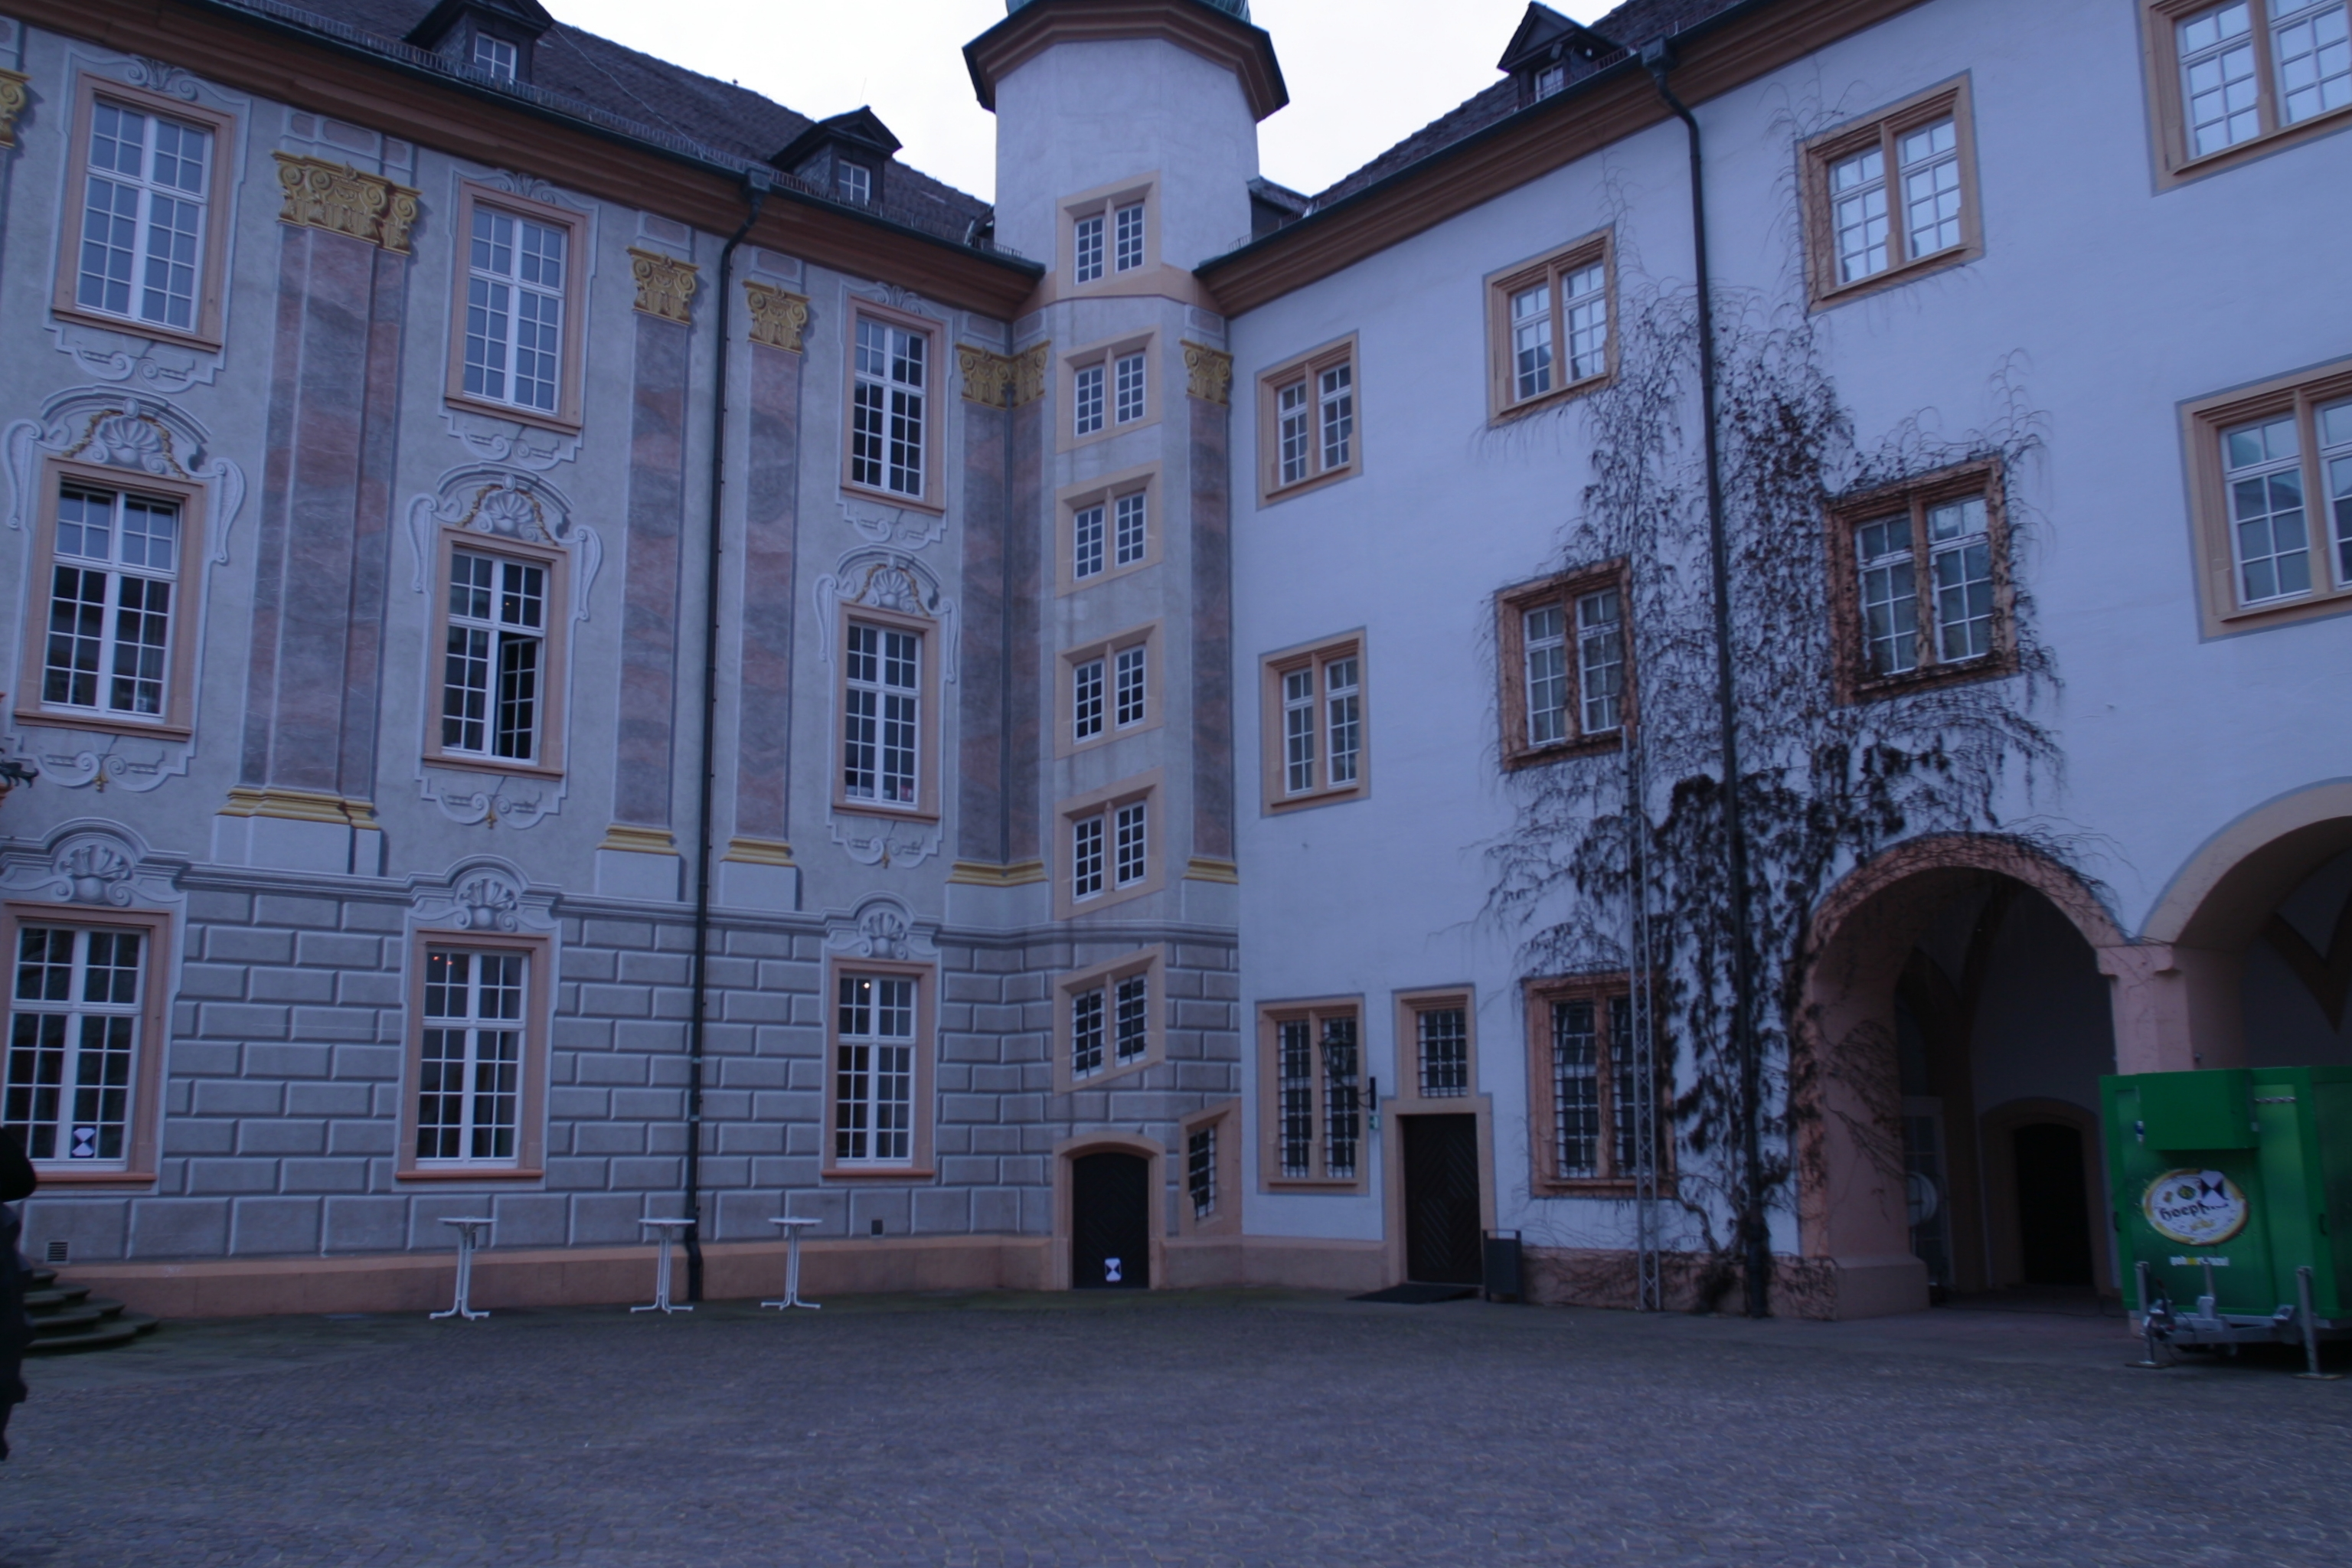
\includegraphics[width=\textwidth]{../../Project_3DAR/images/Testing/fountain-P11/0000.jpg}
     \end{subfigure}
     \hfill
     \begin{subfigure}[b]{0.3\textwidth}
         \centering
         \includegraphics[width=\textwidth]{../../Project_3DAR/images/Testing/fountain-P11/0004.jpg}
     \end{subfigure}
     \hfill
     \begin{subfigure}[b]{0.3\textwidth}
         \centering
         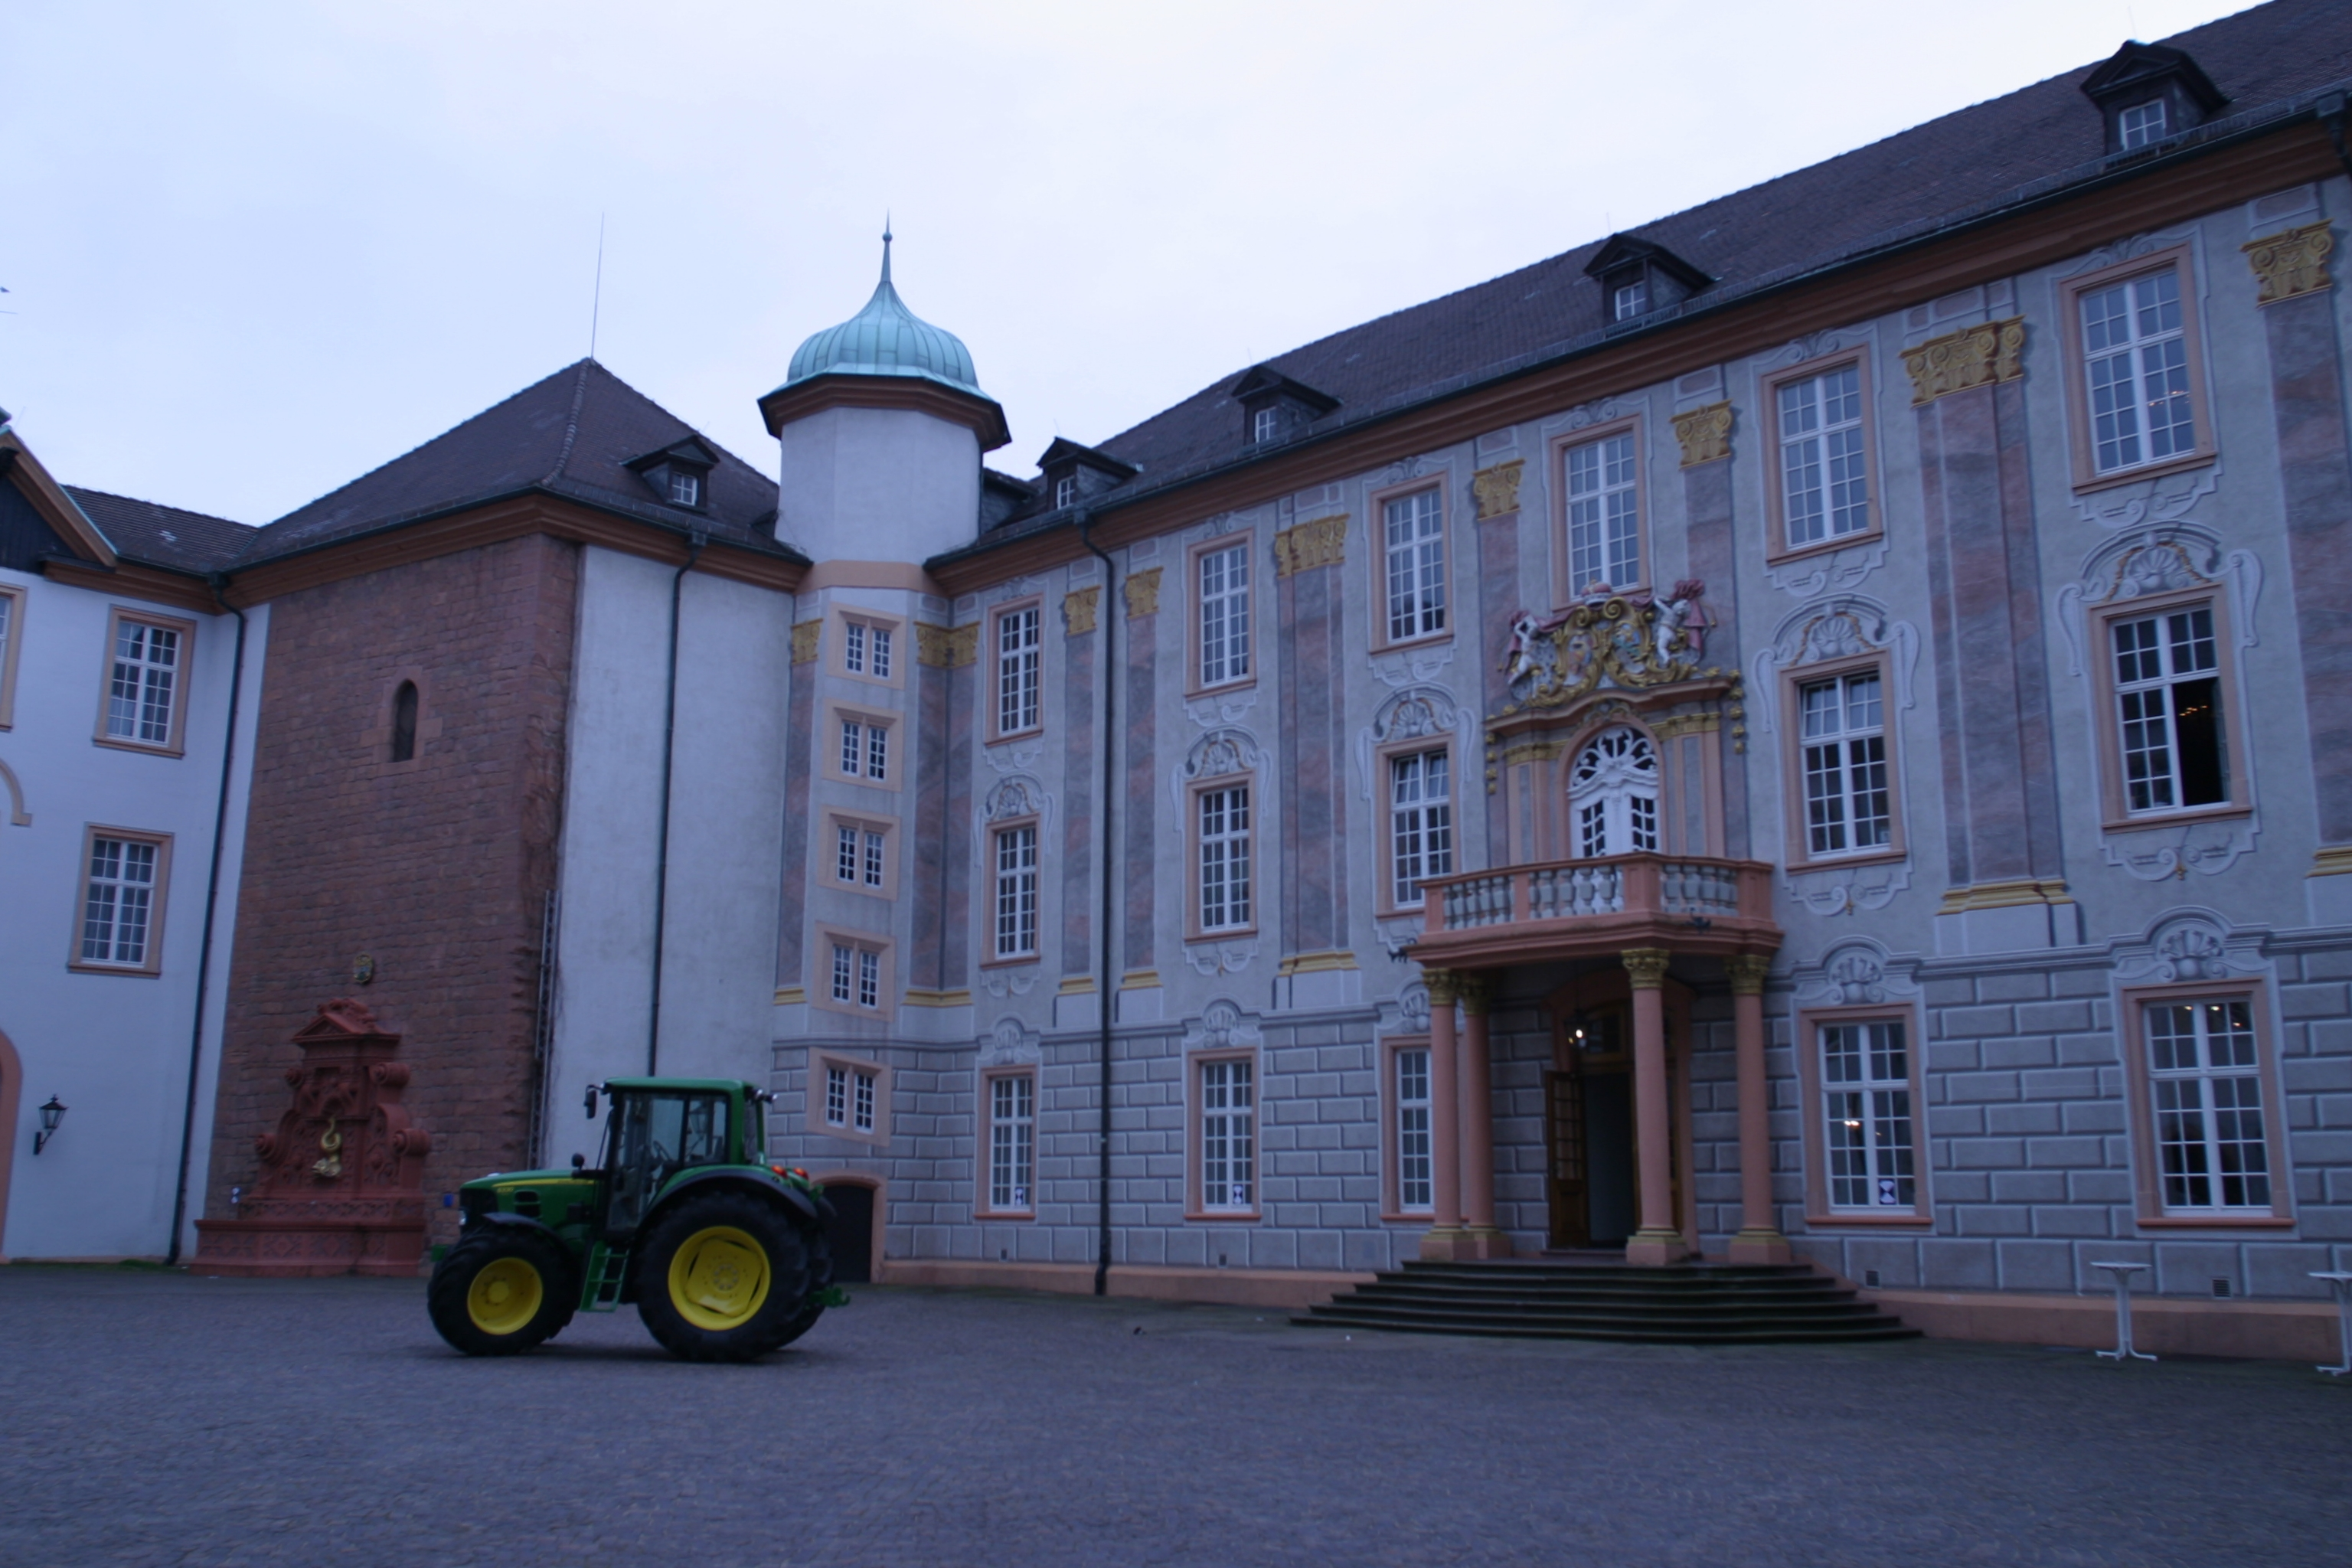
\includegraphics[width=\textwidth]{../../Project_3DAR/images/Testing/fountain-P11/0008.jpg}
     \end{subfigure}
        \caption{samples from Fountain-P11 dataset.}
        \label{fig:fountain}
\end{figure}

\begin{figure}[H]
     \centering
     \begin{subfigure}[b]{0.3\textwidth}
         \centering
         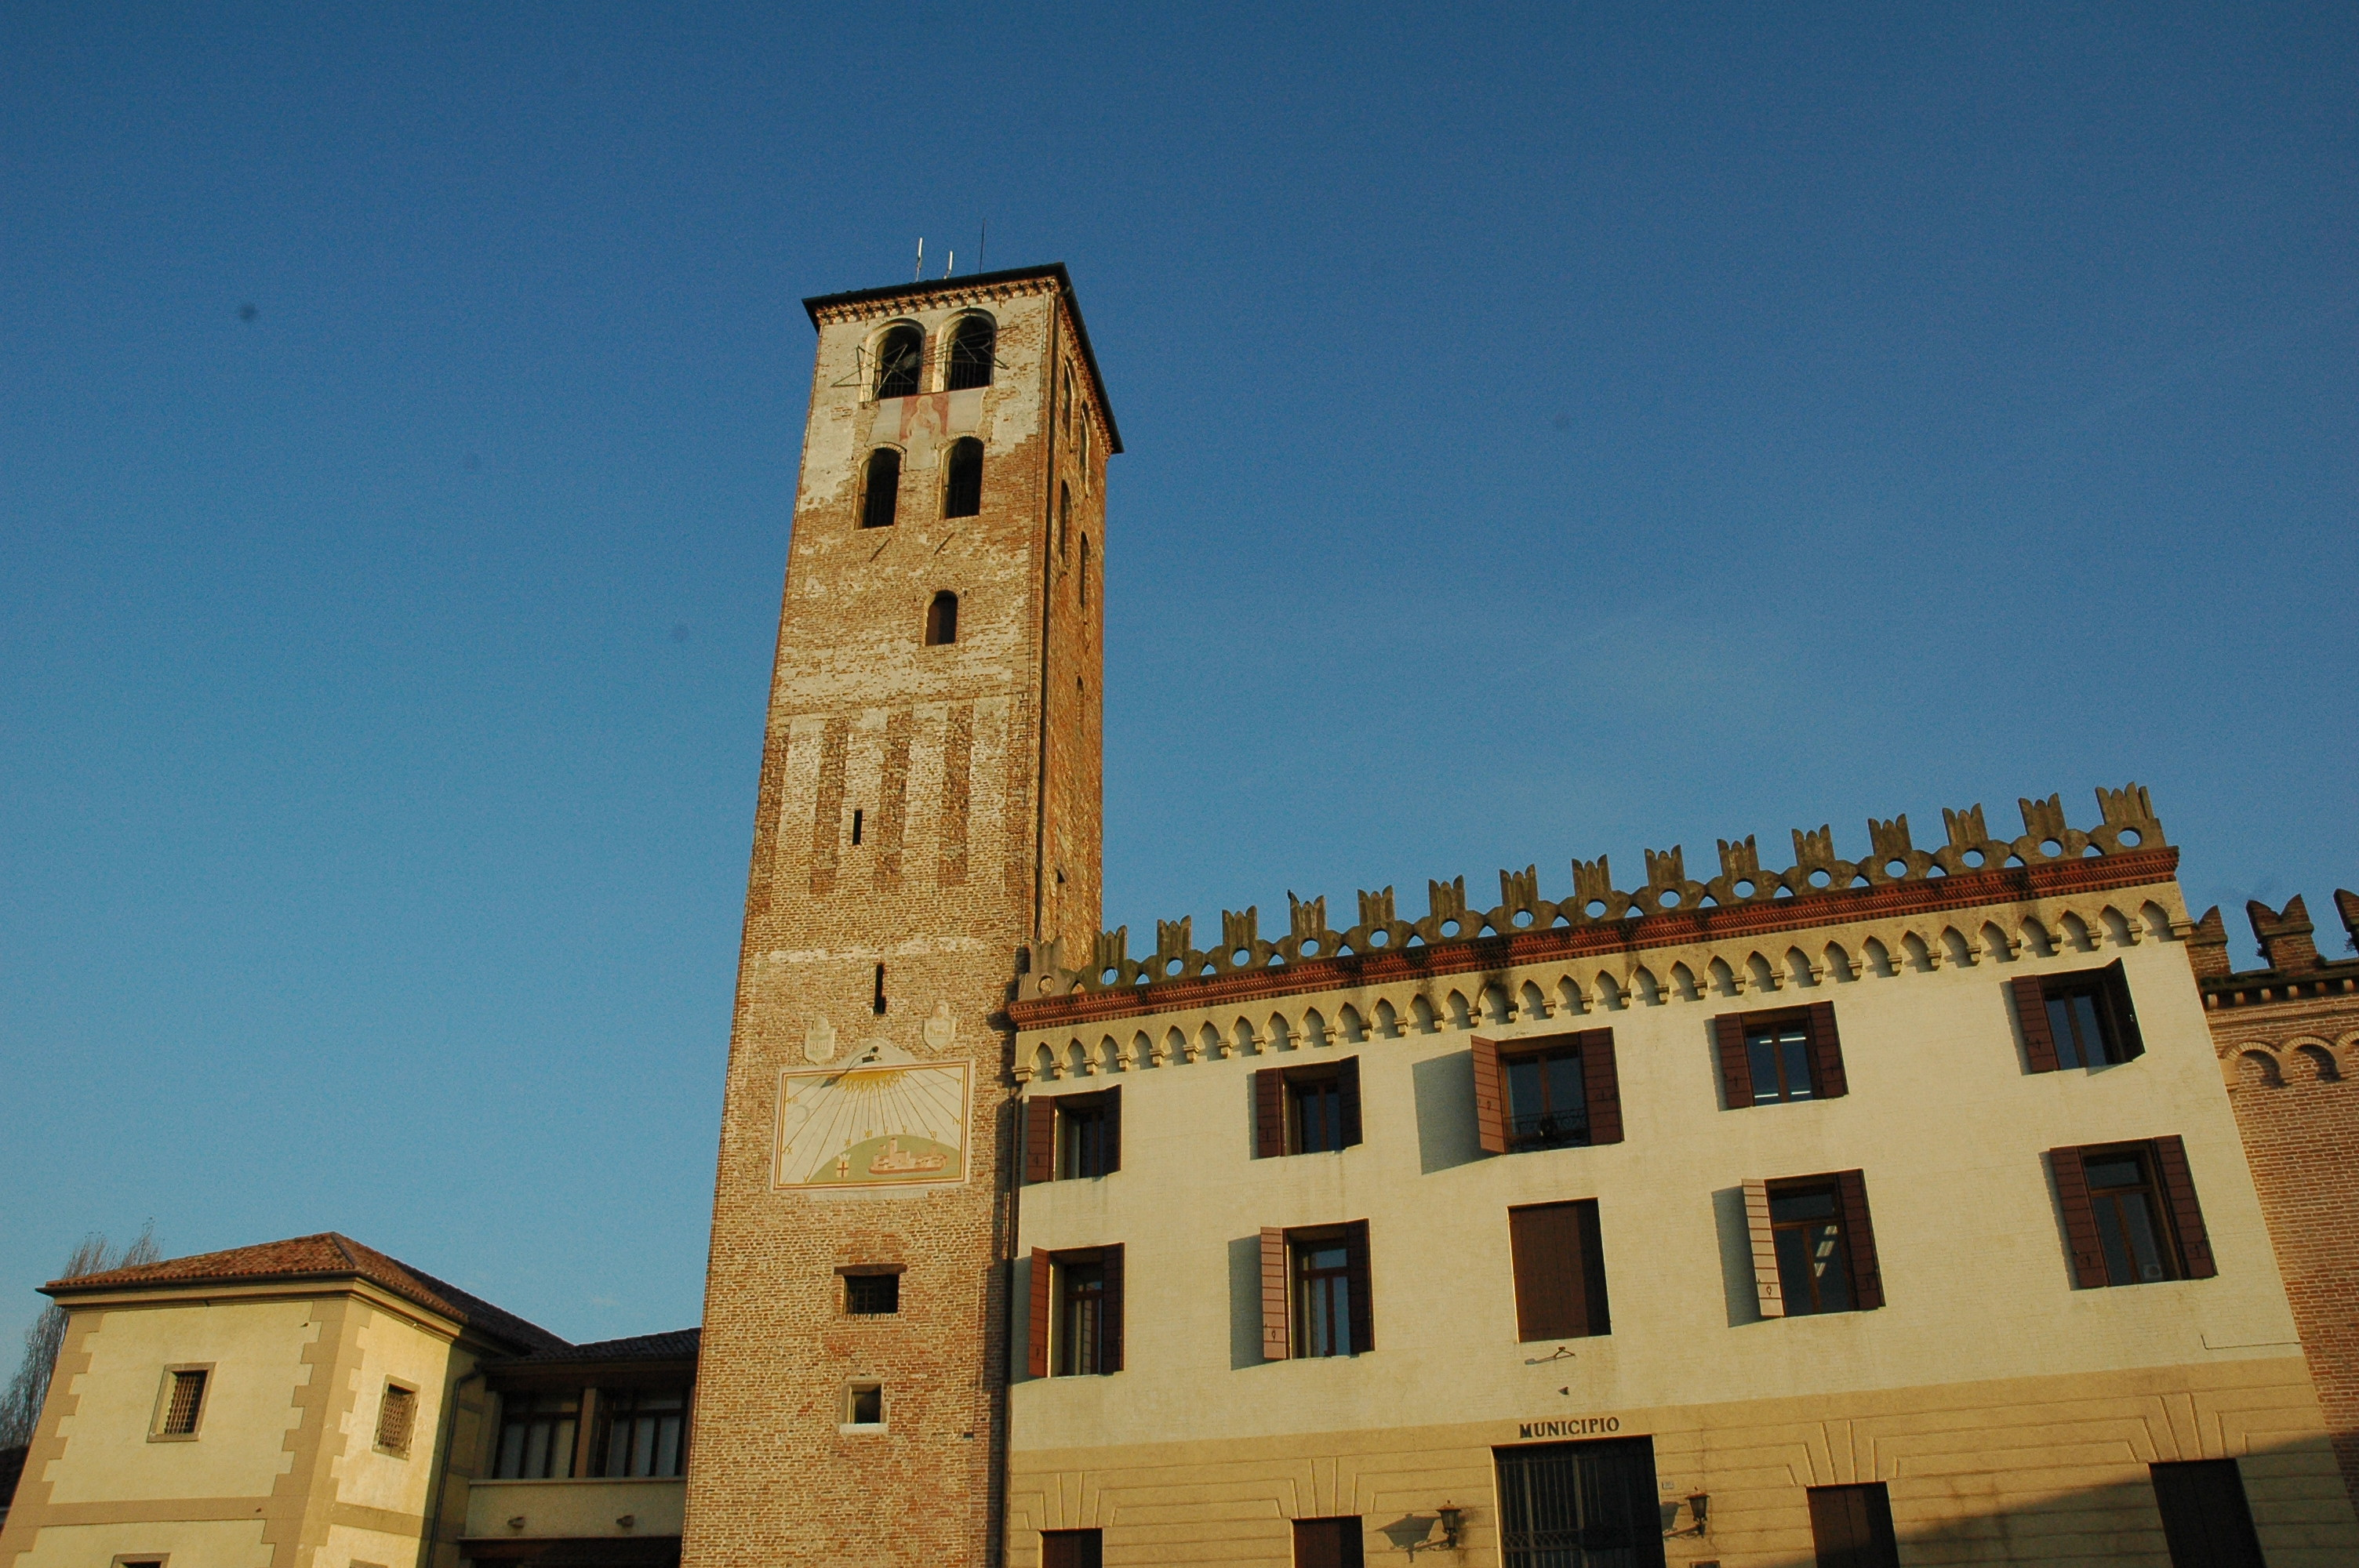
\includegraphics[width=\textwidth]{../../Project_3DAR/images/Testing/tisoDataset/img16c2.jpg}
     \end{subfigure}
     \hfill
     \begin{subfigure}[b]{0.3\textwidth}
         \centering
         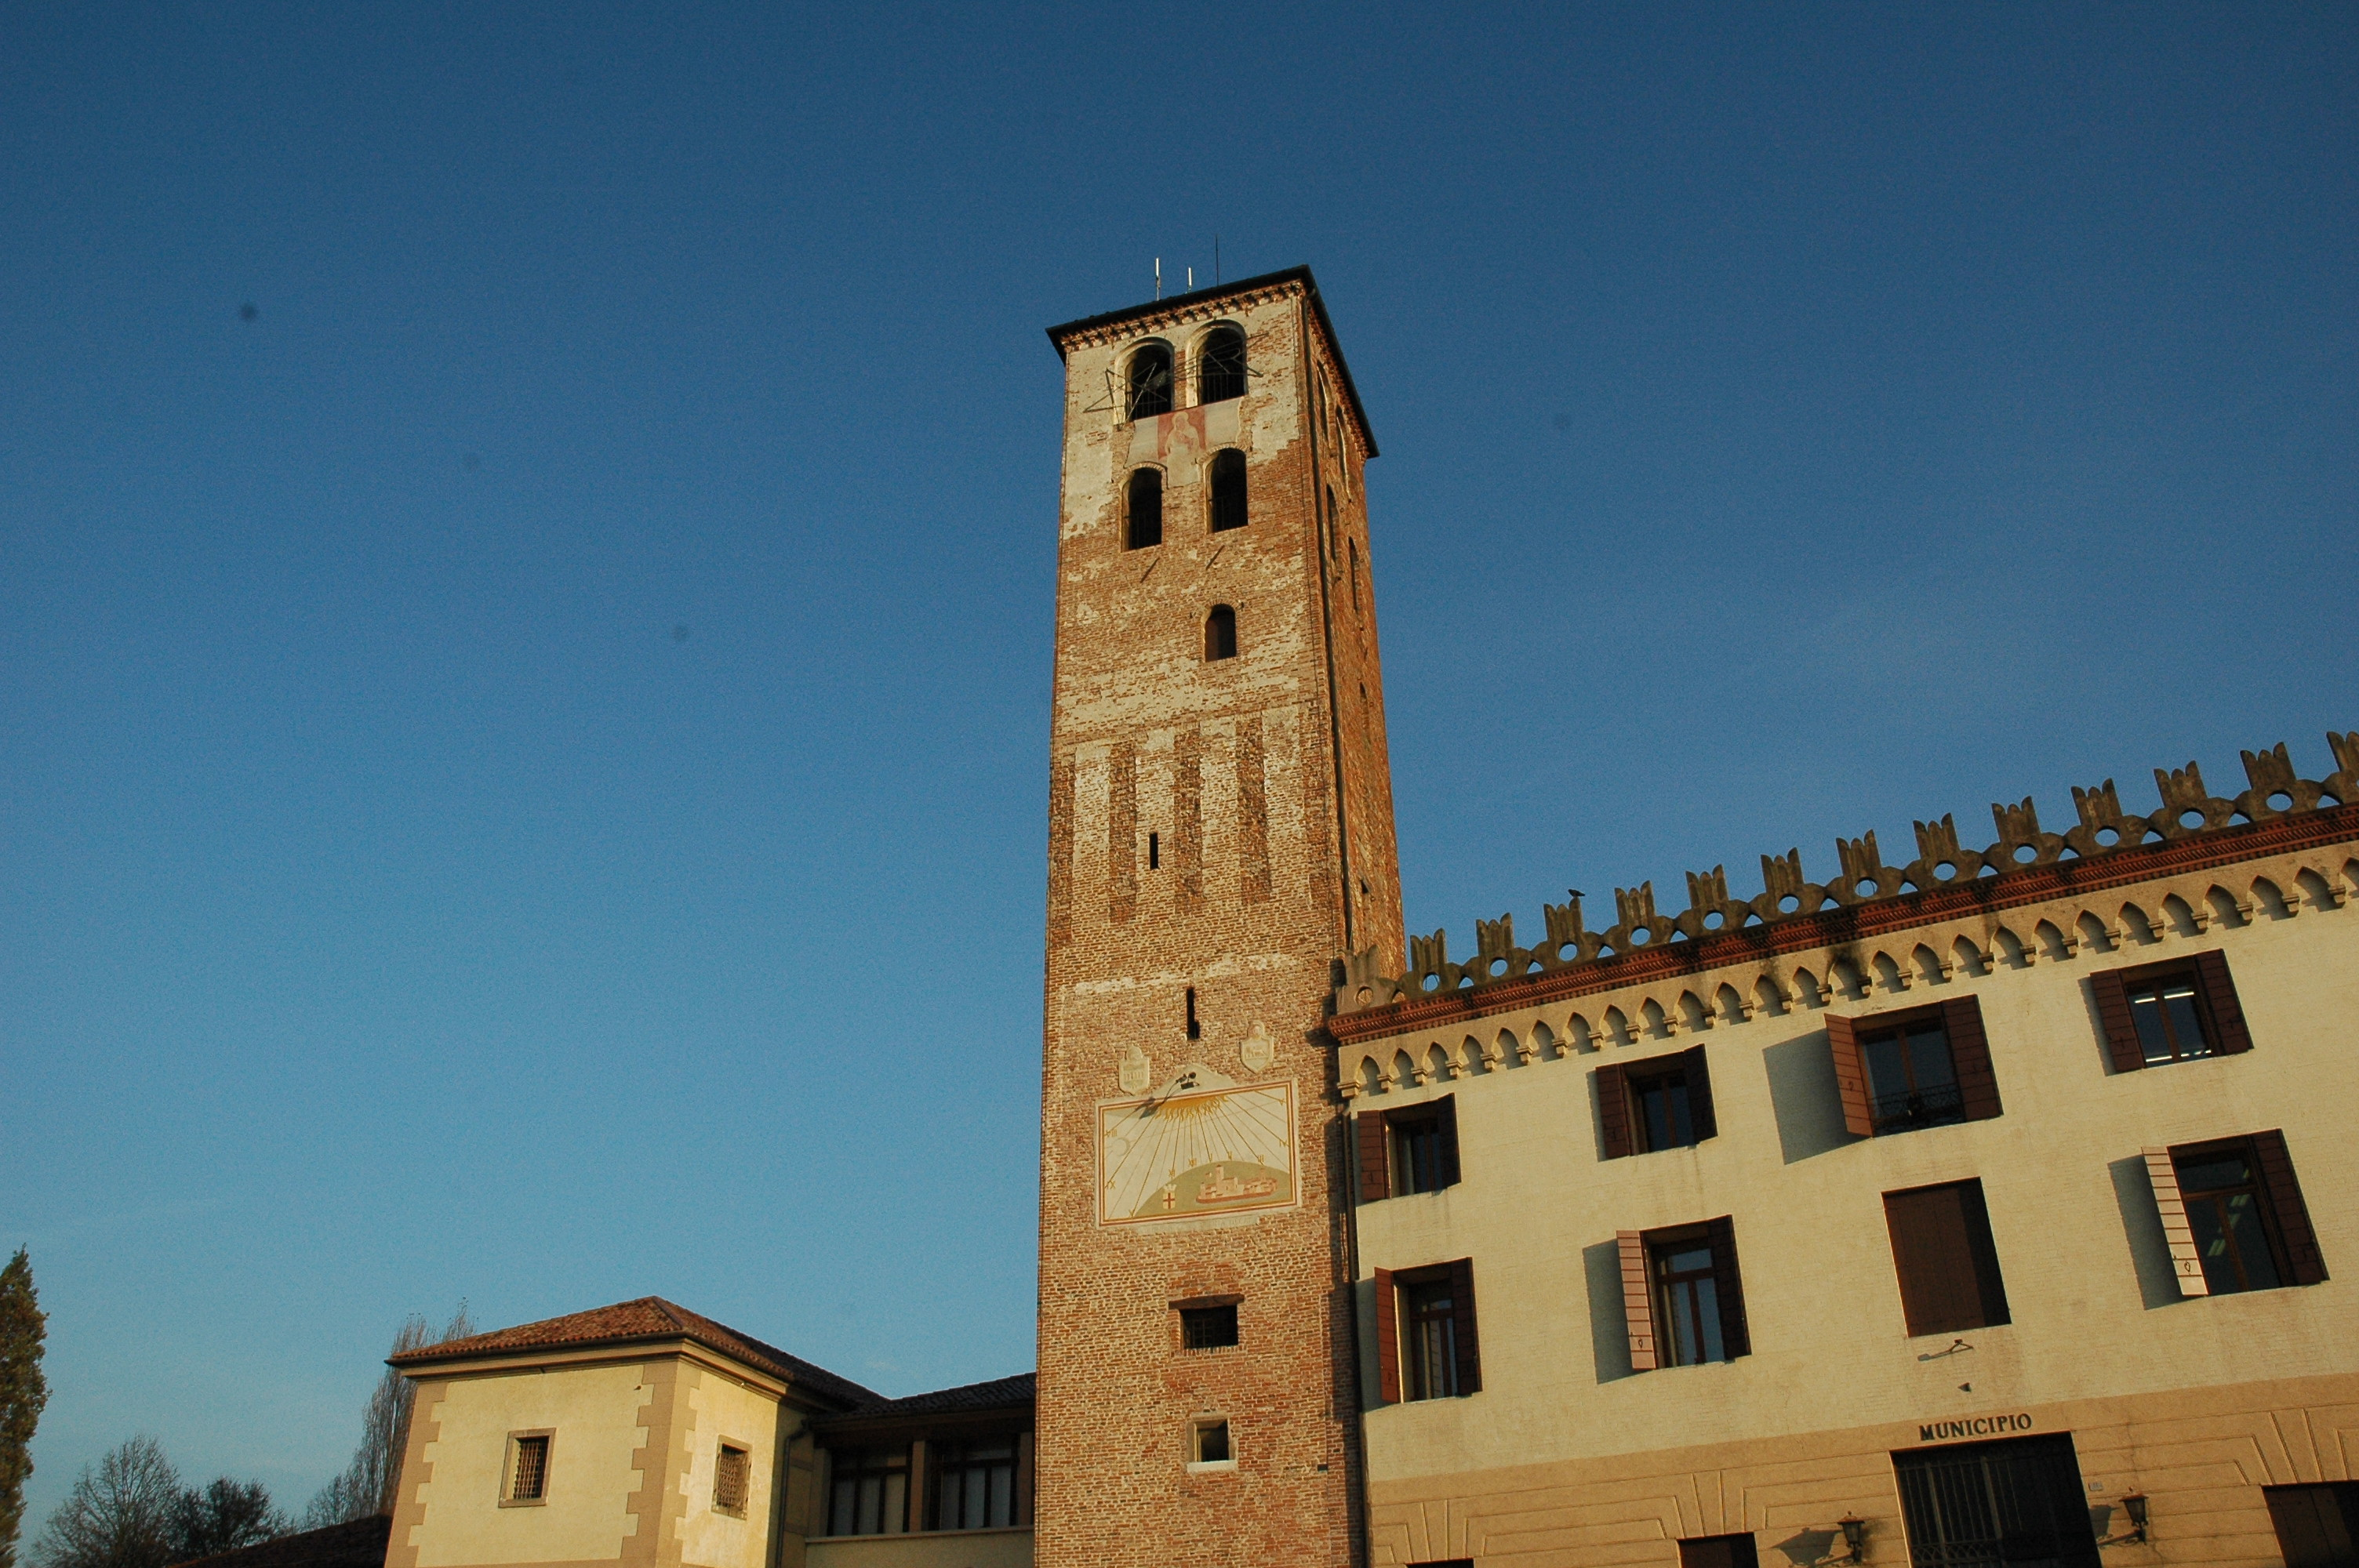
\includegraphics[width=\textwidth]{../../Project_3DAR/images/Testing/tisoDataset/img18c2.jpg}
     \end{subfigure}
     \hfill
     \begin{subfigure}[b]{0.3\textwidth}
         \centering
         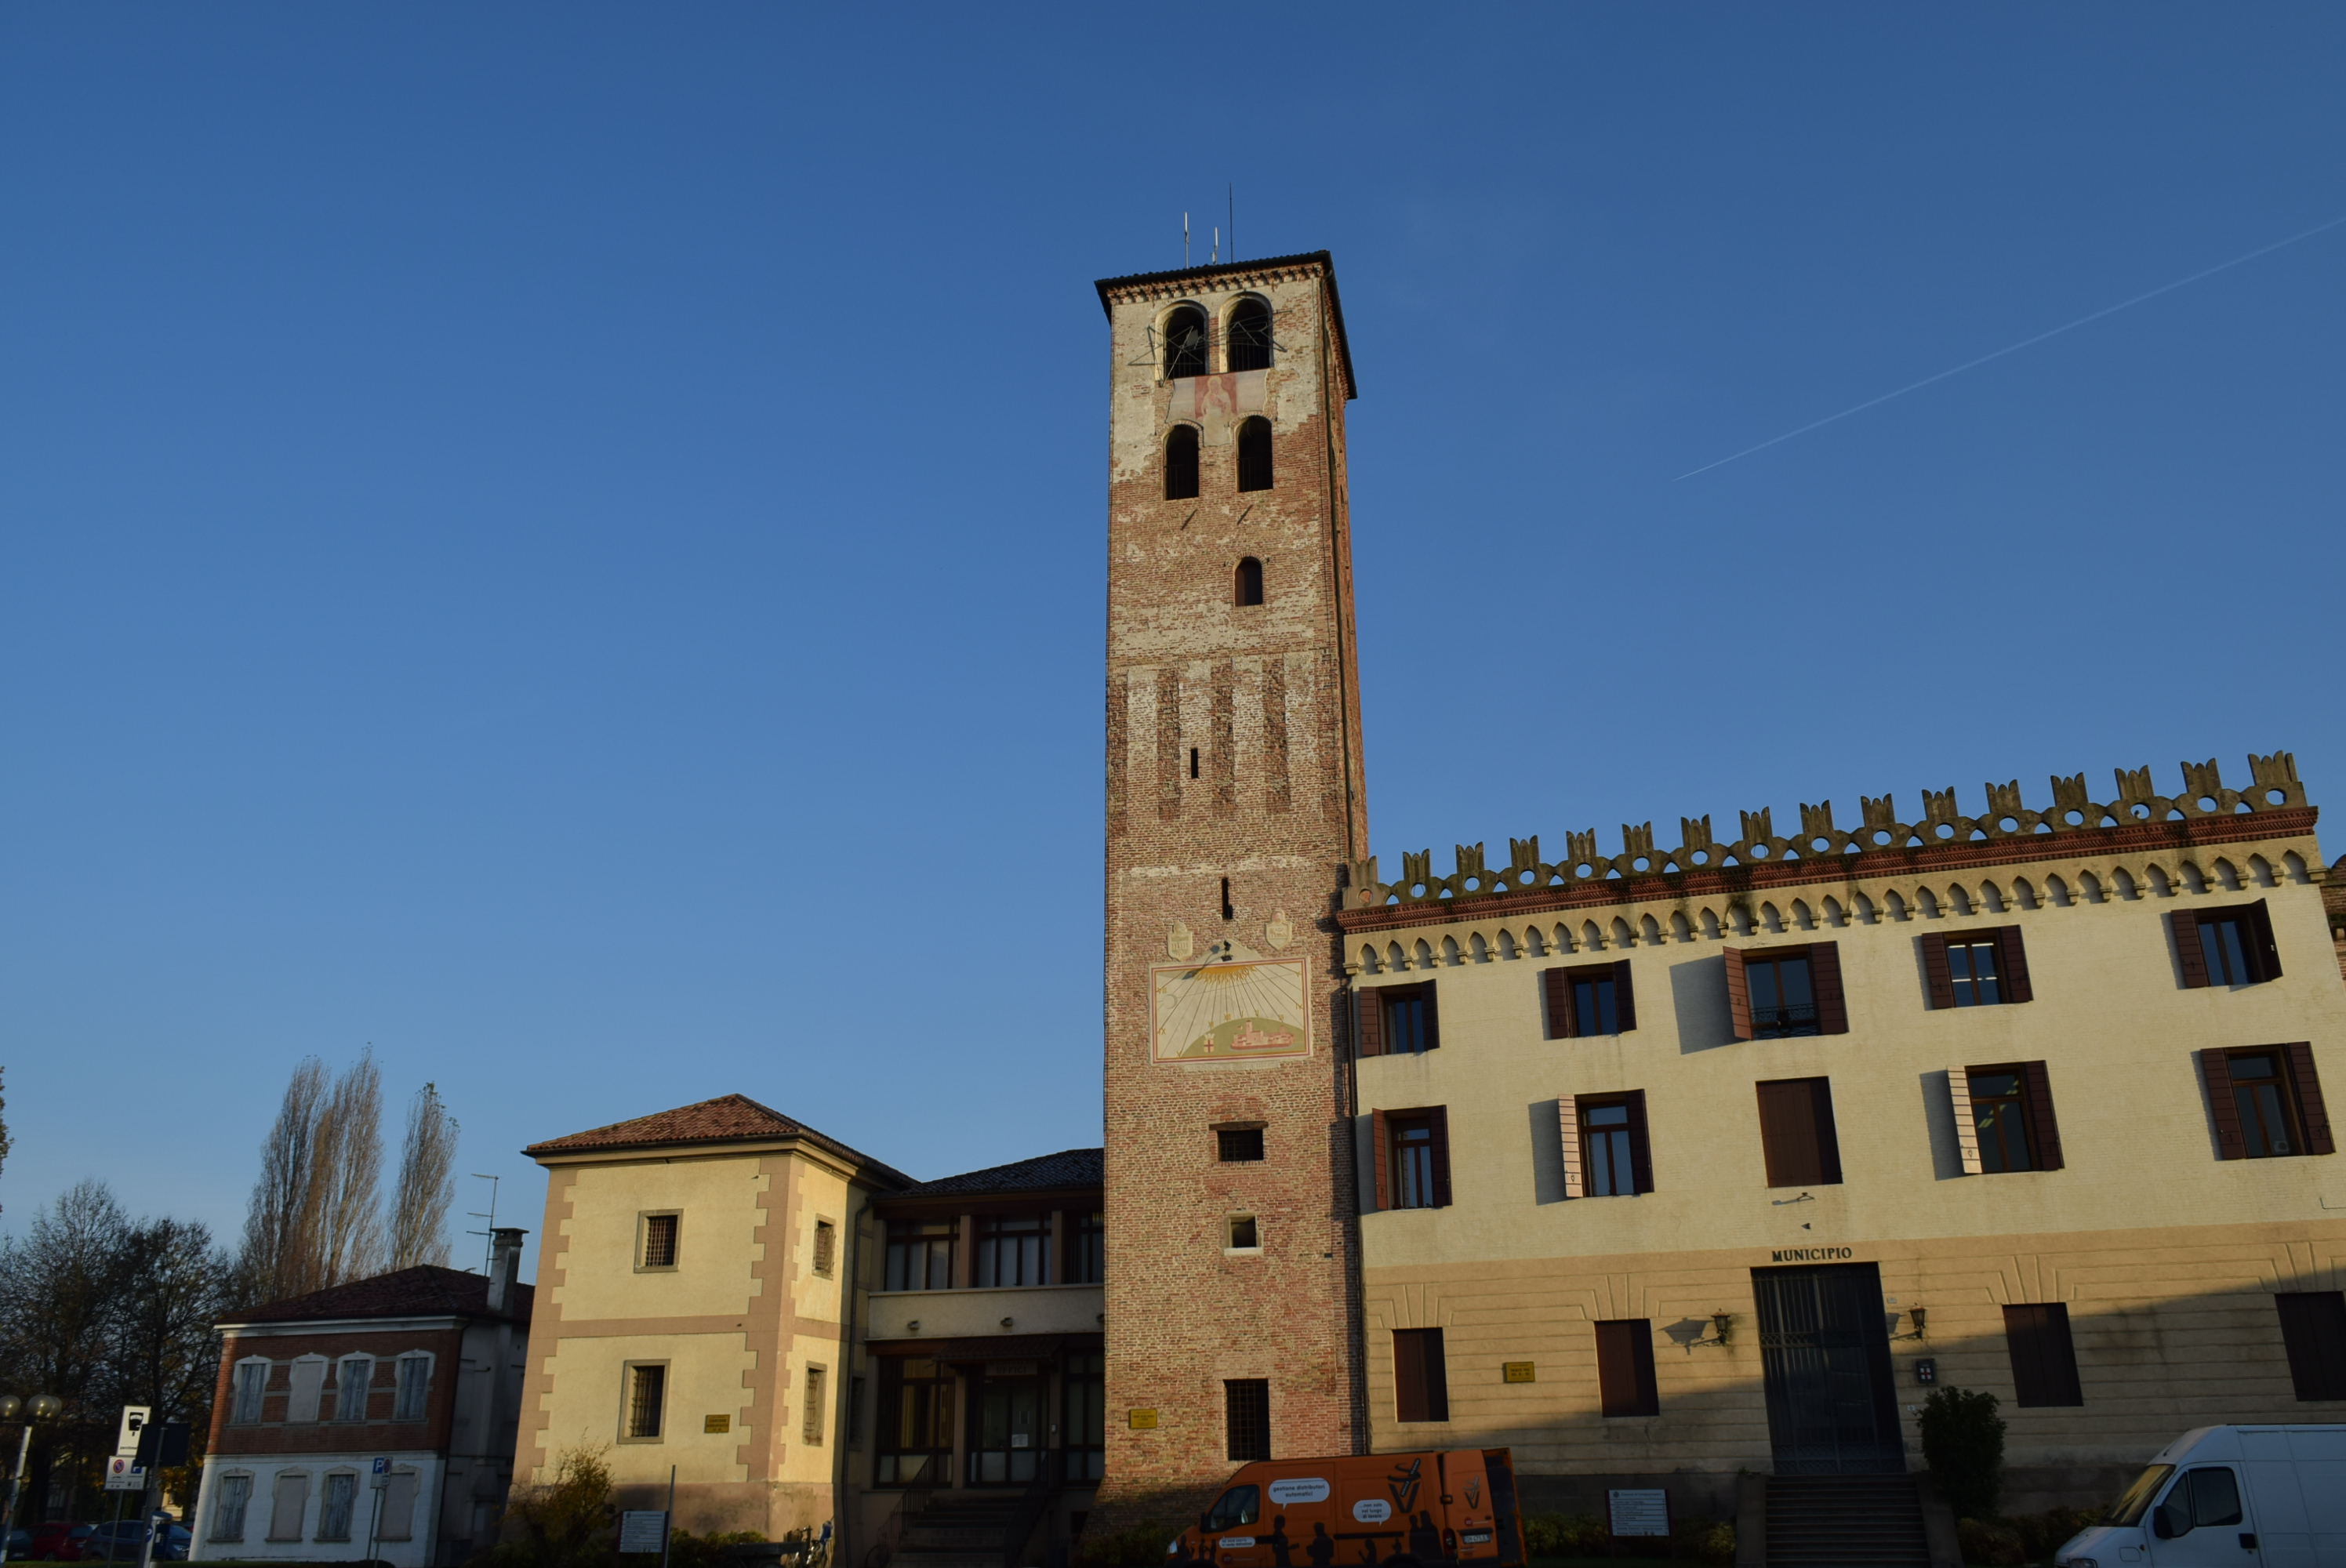
\includegraphics[width=\textwidth]{../../Project_3DAR/images/Testing/tisoDataset/img26c3.jpg}
     \end{subfigure}
        \caption{samples from Tiso dataset.}
        \label{fig:tiso}
\end{figure}

